%%%%%%%%%%%%%%%%%%%%%%%%%%%%%%%%%%%%%%%%%%
%% Short Sectioned Assignment
%% LaTeX Template
%% Version 1.0 (5/5/12)
%%%%%%%%%%%%%%%%%%%%%%%%%%%%%%%%%%%%%%%%%%
%
%%----------------------------------------------------------------------------------------
%%	PACKAGES AND OTHER DOCUMENT CONFIGURATIONS
%%----------------------------------------------------------------------------------------
%
%\documentclass[paper=a4, fontsize=11pt]{scrartcl}
%
%\usepackage[utf8]{inputenc} 
%\usepackage[T1]{fontenc}
%\usepackage[french]{babel}
%\usepackage{amsmath,amsfonts,amsthm}
%
%\usepackage{algorithm}
%\usepackage{algorithmic}
%
%\usepackage{graphicx}
%\usepackage{epstopdf}
%
%\usepackage{lipsum} % Used for inserting dummy 'Lorem ipsum' text into the template
%
%\usepackage{sectsty} % Allows customizing section commands
%\allsectionsfont{\centering \normalfont\scshape} % Make all sections centered, the default font and small caps
%
%\allsectionsfont{\centering \normalfont\scshape} % Make all sections centered, the default font and small caps
%
%\usepackage{fancyhdr} % Custom headers and footers
%\pagestyle{fancyplain} % Makes all pages in the document conform to the custom headers and footers
%\fancyhead{} % No page header - if you want one, create it in the same way as the footers below
%\fancyfoot[L]{} % Empty left footer
%\fancyfoot[C]{} % Empty center footer
%\fancyfoot[R]{\thepage} % Page numbering for right footer
%\renewcommand{\headrulewidth}{0pt} % Remove header underlines
%\renewcommand{\footrulewidth}{0pt} % Remove footer underlines
%\setlength{\headheight}{13.6pt} % Customize the height of the header
%
%\numberwithin{equation}{section} % Number equations within sections (i.e. 1.1, 1.2, 2.1, 2.2 instead of 1, 2, 3, 4)
%\numberwithin{figure}{section} % Number figures within sections (i.e. 1.1, 1.2, 2.1, 2.2 instead of 1, 2, 3, 4)
%\numberwithin{table}{section} % Number tables within sections (i.e. 1.1, 1.2, 2.1, 2.2 instead of 1, 2, 3, 4)
%
%\setlength\parindent{0pt} % Removes all indentation from paragraphs - comment this line for an assignment with lots of text
%\usepackage{todonotes}
%%\usepackage[disable]{todonotes}
%\usepackage{amsthm}
%
%%----------------------------------------------------------------------------------------
%%	TITLE SECTION
%%----------------------------------------------------------------------------------------
%
%\newcommand{\horrule}[1]{\rule{\linewidth}{#1}}
%
%\title{	
%\normalfont \normalsize 
%\textsc{Ecole Polytechnique de Louvain} \\ [25pt]
%\horrule{0.5pt} \\[0.4cm] 
%\huge LINMA2111 Algorithmes et complexité \\ CM 7
%\horrule{0.5pt} \\[0.4cm]
%}
%
%\author{Mélanie Sedda - Benoît Sluysmans} 
%
%\date{\normalsize\today}
%\begin{document}
%
%\maketitle


Let's see an (inefficient) method to compute $\pi$:

\textit{THEOREM (Buffon):} If I throw randomly a needle of length 1 on a floor with planks of width 2, the probability of crossing a crack (i.e. overlap two tracks) is $\frac{1}{\pi}$ (see figure \ref{needles}).


\begin{figure}[h]
\centering
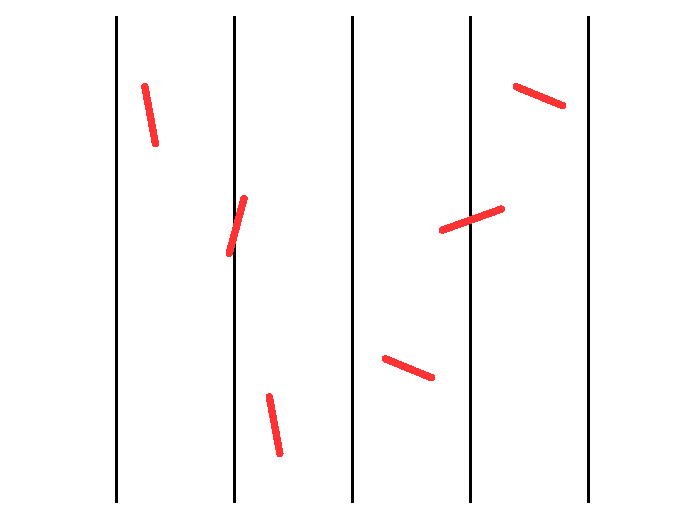
\includegraphics[scale=0.7]{images/needles.eps}
\caption{Needles of length 1 crossing cracks of width 2}
\label{needles}
\end{figure}

\textit{PROOF:}
\begin{enumerate}
\item Trigo + calculus: integrate over all angles and horizontal coordinates of needles.
\item Consider a needle of length $l$.
$E_l := $ expected number of cracks crossed by the needle $= \mathbb{E}(X_l)$, where $X_l$ is the number of cracks crossed. We have
$$
E_{2l} = \mathbb{E}(X_{2l}) = \mathbb{E}(X_l^1+X_l^2) = \mathbb{E}(X_l^1) + \mathbb{E}(X_l^2) = E_l + E_l = 2E_l
$$
More generally, $E_{l_1+l_2} = E_{l_1} + E_{l_2}$. So we see it follows a linear form: $E_l = \alpha l$, for some $\alpha$.\\
If $l=1$, as it never crosses twice, we can write 
$$
X_l = \left\{
      \begin{aligned}
        &1 \text{ if the needle crosses a crack}& \\
        &0 \text{ otherwise}& \\
      \end{aligned}
    \right.
$$
    So $E_l$ is the probability to cross a crack. Now we have to proof that $\alpha = \frac{1}{\pi}$.\\
Let be even more general: let's bend the needle. We have
$$
\mathbb{E}(\text{number of cracks crossed}) = E_{l_1} + E_{l_2}
= \alpha (l_1 + l_2)
= \alpha l
$$
with $l$ the total length of the needle. We can bend it several times...
$$
\mathbb{E}(\text{number of cracks crossed}) = \alpha \sum_i l_i = \alpha l
$$

\begin{figure}[h]
\centering
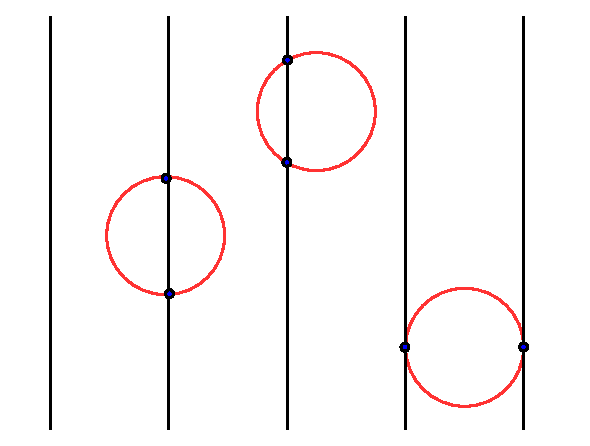
\includegraphics[scale=0.7]{images/circles.eps}
\caption{Circular needles of radius 1 crossing cracks of width 2}
\label{circles}
\end{figure}

In the limit, for a curved needle of length $l$, we always have $\mathbb{E}(\text{number of cracks crossed}) = \alpha l$. To fix $\alpha$, let's look at a circular needle of radius $1$, such that $E_l=2$, always (see figure \ref{circles})! We can write $E_{2\pi} = 2$, but $E_{2\pi} = \alpha 2 \pi$, and we conclude with $\alpha = \frac{1}{\pi} $.
\end{enumerate} \qed

We can then develop an algorithm to compute $\pi$:
\begin{itemize}
\item Throw a needle $n$ times on the floor (as in Buffon's theorem)
\item Count how many times a crack is crossed (define this number as $k$)
\item $\pi = \frac{n}{k}$
\end{itemize}

Accuracy of this algorithm? Let's look at its variance. Let
$$
X_i = \left\{
      \begin{aligned}
        &1 \text{ if the } i^{th} \text{ needle crosses a crack}& \\
        &0 \text{ otherwise}& \\
      \end{aligned}
    \right.
$$
As we have $\mathbb{E}(X_i)=\frac{1}{\pi}$ and $Var(X_i) = \frac{1}{\pi}(1-\frac{1}{\pi})$ and the $X_i$ are independant, it follows that
\begin{eqnarray*}
\mathbb{E}(\frac{\sum_i X_i}{n}) &=& \frac{1}{\pi} \\
Var(\frac{\sum_i X_i}{n}) &=& \frac{n \frac{1}{\pi}(1-\frac{1}{\pi})}{n^2} = \frac{1}{n}\frac{1}{\pi}(1-\frac{1}{\pi})
\end{eqnarray*}
We can now compute the standard deviation $\sigma = \frac{1}{\sqrt{n}}\sqrt{\frac{1}{\pi}(1-\frac{1}{\pi})}$ = typical error in $\frac{1}{\pi}$:
$$
\frac{k}{n} \in [\frac{1}{\pi}-\frac{2}{\sqrt{n}}\sqrt{\frac{1}{\pi}(1-\frac{1}{\pi})}; \frac{1}{\pi}+\frac{2}{\sqrt{n}}\sqrt{\frac{1}{\pi}(1-\frac{1}{\pi})}]
$$
with 95\% probability.\\
\textit{Remarks:}
\begin{itemize}
\item To gain one digit of accuracy, you need 100 times more throws: not good.
\item The result is possibly wrong, with some probability (here 5\%).
\end{itemize}

%\end{document}